\documentclass[a4paper,titlepage]{book}
\usepackage{frontespizio}

\usepackage[utf8]{inputenc} % set input encoding (not needed with XeLaTeX)

%%% Examples of Article customizations
% These packages are optional, depending whether you want the features they provide.
% See the LaTeX Companion or other references for full information.

%%% PAGE DIMENSIONS
\usepackage{geometry} % to change the page dimensions
\geometry{a4paper} % or letterpaper (US) or a5paper or....
% \geometry{margin=2in} % for example, change the margins to 2 inches all round
% \geometry{landscape} % set up the page for landscape
%   read geometry.pdf for detailed page layout information

\usepackage{graphicx} % support the \includegraphics command and options

% \usepackage[parfill]{parskip} % Activate to begin paragraphs with an empty line rather than an indent

%%% PACKAGES
\usepackage{booktabs} % for much better looking tables
\usepackage{array} % for better arrays (eg matrices) in maths
\usepackage{paralist} % very flexible & customisable lists (eg. enumerate/itemize, etc.)
\usepackage{verbatim} % adds environment for commenting out blocks of text & for better verbatim
\usepackage{subfig} % make it possible to include more than one captioned figure/table in a single float
% These packages are all incorporated in the memoir class to one degree or another...
\usepackage[italian]{babel}
\usepackage{amsmath}
\usepackage[]{algorithm2e}


%%% HEADERS & FOOTERS
\usepackage{fancyhdr} % This should be set AFTER setting up the page geometry
\pagestyle{fancy} % options: empty , plain , fancy
\renewcommand{\headrulewidth}{0pt} % customise the layout...
\lhead{}\chead{}\rhead{}
\lfoot{}\cfoot{\thepage}\rfoot{}


\begin{document}


\begin{frontespizio}
\Universita{Verona}
\Dipartimento{Informatica}
\Corso[Laurea Magistrale]{Ingegneria e Scienze Informatiche}
\Titoletto{Tesi di laurea magistrale}
\Titolo{Generazione automatica di modelli SystemC RTL di hardware riconfigurabile dinamicamente}
\Candidato[VR386687]{Enrico Giordano}
\Relatore{Prof. Graziano Pravadelli}
\Annoaccademico{2015-2016}
\end{frontespizio}


\chapter*{Introduzione}

Il flusso di progettazione standard di un sistema embedded si divide in tre step: analisi, progettazione e sintesi; questo flusso mira ad avere un sistema specifico per una situazione particolare e alla sintesi finale di tale sistema il meno generale possibile, in modo da renderlo massimamente performante per quel particolare ambiente.

Con questa tesi, si vuole proporre un approccio alternativo il cui mezzo è l'utilizzo di hardware metamorfico e quindi di una particolare tecnica di progettazione basata sulla ``configurabilità parziale'' della tecnologia delle FPGA. Usando questo mezzo, si vuole progettare un sistema che presenta aspetti embedded (quindi specifici per il target finale) e aspetti più generici e, calato in un contesto particolare, sarà in grado di modificarsi in base alle esigenze ed essere più performante per il contesto in cui viene utilizzato, risparmiando energia, computazioni e memoria. Basandosi sul concetto di ``evoluzione'', secondo cui un oggetto si modifica in base all'ambiente, si otterrà per ogni ambiente un particolare sistema embedded.

Si presenteranno quindi, a livello descrittivo, le diverse tecniche di configurabilità parziale, introducendo poi un modello di progettazione che mira ad un approccio standardizzato per i futuri sviluppi di questa idea, per poi provare il tutto su un caso di studio reale che possa dimostrare i benefici di questa tecnologia e tecnica di progettazione.


\tableofcontents

\chapter{Tecnologia attuale del silicio}
Attualmente esistono 3 tecnologie differenti riguardo l'utilizzo del silicio per scopi computazionali: Hardware General Purpoise, Hardware Embedded e Hardware Riprogrammabile. Queste 3 tipologie differiscono sia per la composizione, sia per la progettazione ma anche per il settore di utilizzo.

\section{Hardware General Purpoise}
Questo tipo di Hardware lo si può trovare in processori e microprocessori utilizzati in strumenti di calcolo generici, come PC, moderni telefoni e televisori. La caratteristica peculiare di questi è la generalità: non essendo stati progettati per un sistema specifico, devono permettere di eseguire più operazioni possibili ed essere riprogrammati a piacimento, al limite delle loro potenzialità.

Questi sono composti da un'architettura standard,  rappresentata nella figura  \ref{fig:0}, e viene implementata in ogni CPU, ovvero ciò che implementa questa tecnologia.

\begin{figure}
\centering
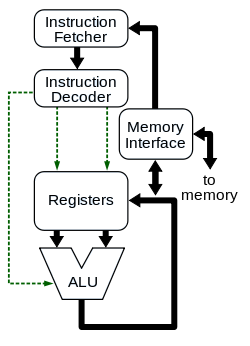
\includegraphics[scale=1]{cpu.png}
\caption{Architettura di una CPU}\label{fig:0}
\end{figure}

Il ciclo di vita di questo hardware è contraddistinto da 3 fasi: fetch, decode, exec; ogni fase è contraddistinta da un insieme di componenti interni utilizzati. La fase di ``fetch'' consiste nel caricare l'istruzione corrente per essere eseguita; la fase di ``decode'' fa in modo che tutti i valori siano disponibili per il calcolo e che l'istruzione possa essere eseguita correttamente impostando i registri interni; la fase di ``exec'' permette, tramite i componenti di memoria e di calcolo (registri e ALU), di eseguire l'istruzione.

Questo tipo di hardware è molto utile per implementare sistemi generici: la filosofia alla base di questa tecnologia è l'utilizzo più generico possibile, mettendo in secondo piano l'ottimizzazione e il consumo, oltre al costo che cerca di stare relativamente nelle politiche di mercato.

\section{Hardware Embedded}
Questo tipo di Hardware è contraddistinto dalla specificità dei suoi componenti interni in base al suo utilizzo; infatti si cerca di utilizzare questo hardware in ambienti o condizioni specifiche, in cui sono richieste operazioni particolari ma soprattutto è necessario ridurre i costi e il consumo dell'applicazione finale.
La tecnologia che rappresenta questo tipo di hardware è una ASIC e difficilmente si trova un'architettura standard, proprio perché l'architettura è specifica per un certo comportamento. Esistono in commercio dei sistemi embedded basati su microprocessori RISC, come ad esempio i Cortex-M della ARM, che hanno un'architettura molto simile a quella delle CPU. In generale comunque ogni ASIC è diversa, in quanto viene mappato su silicio uno specifico algoritmo o un'architettura più complessa.

Un' ASIC deve costare il meno possibile e deve consumare il meno possibile, in base alle esigenze richieste; ovviamente potrà eseguire solo il compito per cui è stata progettata; ha quindi una filosofia di progettazione opposta a quella dell'Hardware General Purpoise.

\section{Hardware Riprogrammabile}
L'ultimo tipo di Hardware è quello riprogrammabile, ovvero permette di essere configurato a livello di celle di memoria più volte per implementare diversi comportamenti. Di solito viene utilizzato sia in ambito embedded, per permettere più libertà di progettazione e più efficienza, ma anche a scopo sperimentale, perchè è utile per testare un sistema in fase di sviluppo.

\begin{figure}
\centering
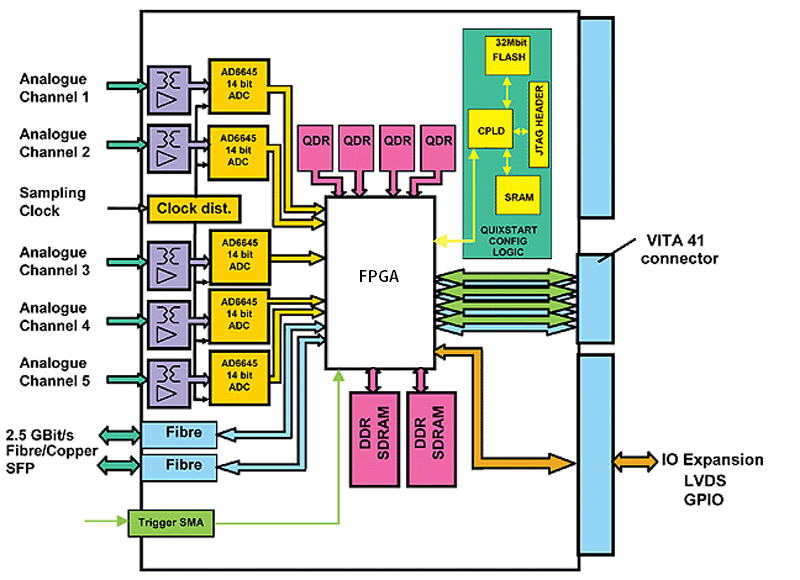
\includegraphics[scale=0.6]{fpga.png}
\caption{Architettura di una FPGA}\label{fig:00}
\end{figure}

Un esempio di architettura (dipende molto dal modello che si vuole utilizzare) lo si può osservare nella figura \ref{fig:00}: la parte riconfigurabile, denotata con FPGA, consiste in un blocco di celle riconfigurabili, che, in base alla descrizione hardware caricata nella memoria flash, possono cambiare struttura. Attorno alla FPGA sono presenti vari moduli standard che possono servire per il consueto utilizzo in ambito di controlli, ma non sempre sono necessarie, in quanto si possono descrivere all'interno della parte riconfigurabile. Parte necessaria per il funzionamento corretto di una FPGA è la logica di controllo della parte riprogrammabile: deve esserci un hardware dedicato per rimappare questa parte, in modo che il processo di riconfigurazione avvenga più velocemente possibile; questo si occuperà quindi di riconfigurare, in base al bitstream che rappresenta l'hardware, la parte riconfigurabile.

In base al suo utilizzo può assumere aspetti di un hardware general purpoise e di un hardware embedded; essendo una tecnologia piuttosto costosa si cerca di utilizzarla il meno possibile, o almeno solo in fase di test.

\chapter{Hardware Metamorfico e tecnologia associata}

Si vedrà ora nel dettaglio il significato di hardware metamorfico e in particolare la tecnologia che implementa questo concetto. 

\section{Il concetto di Hardware Metamorfico}

Il concetto di ``Hardware Metamorfico'' nasce nei primi anni del 1990, per poi perdere parzialmente interesse in quanto veniva presentato come idea, non come tecnologia pratica. Con questo concetto si intende un tipo di Hardware capace di cambiare il proprio comportamento (``evolvere'') utilizzando un ``metodo'' di riconfigurazione: i termini ``evolvere'' e ``metodo'' non sono mai stati definiti in maniera standard, l'articolo che cerca di porre chiarezza su tutto questo ambito \cite{MS1} focalizza l'attenzione sulle diverse sfaccettature del termine ``evoluzione'', parlando di evoluzione ``intrinseca'' , ``estrinseca'' e ``mixata'', rimandando la definizione ad un articolo scientifico precedente \cite{EIE}.

Questo tipo di Hardware è tipico del mondo naturale, in quanto tutti gli oggetti e gli esseri viventi sono in grado di modificarsi in base all'ambiente che li circonda.

\begin{figure}
\centering
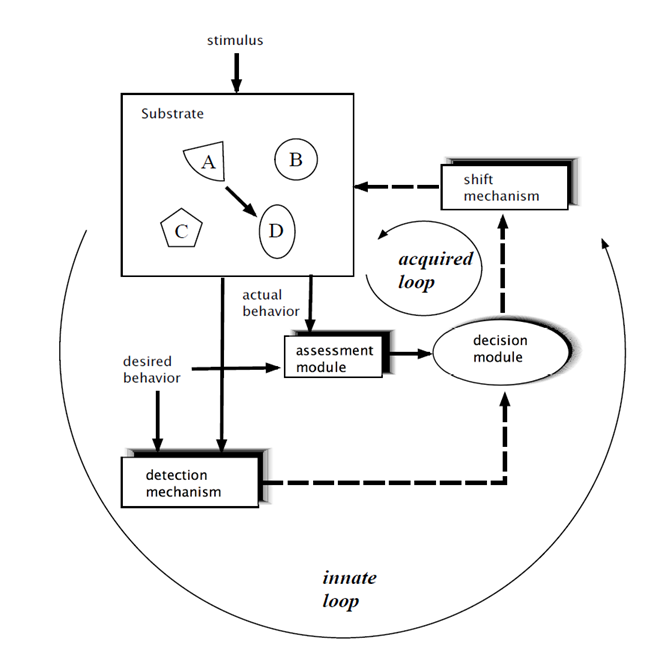
\includegraphics[scale=0.6]{ciclo_evolutivo.png}
\caption{Ciclo evolutivo di un sistema metamorfico}\label{fig:1}
\end{figure}

Il ciclo di vita di un Hardware Metamorfico può essere rappresentato come nella figura \ref{fig:1}: il superciclo che compone questo sistema, chiamato ``ciclo innato'', ha un sotto-ciclo di acquisizione di stimoli, chiamato ``ciclo di acquisizione'', che, tramite il sottostrato di algoritmi di esecuzione, cambia il funzionamento del sistema in base al ``comportamento attuale'' e il ``comportamento desiderato''; con questi dati, tramite un modulo di valutazione degli stimoli e un meccanismo di investigazione (per valutare il comportamento desiderato rispetto al comportamento attuale), viene generato dal modulo di ``decisione'' il risultato che fa modificare l'intero sistema. Il ciclo innato successivamente fa rieseguire questo procedimento, in modo da permettere, potenzialmente all'infinito, la metamorfosi del sistema.

\section{Hardware riconfigurabile}

Per rendere utile l'hardware metamorfico, è necessario trovare una tecnologia che lo rappresenti, in modo da rendere concreto l'utilizzo di tale idea. Per renderla concreta, è necessaria la presenza di un oggetto che possa riprodurre sia il comportamento di silicio, sia il comportamento evolutivo dell'hardware metamorfico. Nel 1985, la Xilinx aveva creato le prime FPGA, rilasciando in commercio il primo modello ``XC2064'', utilizzabile perloppiù per la prototipizzazione di circuiti programmabili. Questa tecnologia sembra prestarsi coerentemente con l'idea di Hardware metamorfico, in quanto è in grado di poter cambiare il proprio comportamento a livello hardware cambiando la propria struttura interna. Il suo carattere riconfigurabile però è stato progettato e utilizzato per la prototipizzazione, non per l'effettivo mutamento di comportamento durante il suo ciclo di vita.

Nei primi anni `90 nasce una tecnica di progettazione chiamata ``Riconfigurabilità'', da qui poi la tecnologia di applicazione, appunto le FPGA. Questa tecnica consiste nell'utilizzare Hardware con tecnologia riprogrammabile che, tramite la memoria messa a disposizione dentro il sistema, riesce a modificare il suo comportamento. Non è un comportamento appreso completamente dall'ambiente, ma è un comportamento previsto e quindi implementato che va a sostituire un comportamento esistente; il ciclo di vita quindi non sarà composto da un vero e proprio ``apprendimento'', ma sarà una modifica prevista dal progettista. Questo può sembrare limitante, in quanto non c'è piena libertà da parte del dispositivo, ma non avrebbe senso far prendere iniziativa a questo (per i principi della computabilità, non sarebbe nemmeno possibile).

Quindi, più precisamente, si più parlare di ``riconfigurabilità parziale'' e ``riconfigurabilità run-time'': il primo termine pone enfasi su la parziale capacità del dispositivo di modificarsi, in quanto ci sarà una parte progettata che non deve modificarsi ma soprattutto perché il dispositivo non si modificherà completamente, avrà delle modifiche consentite prestabilite; il secondo termine indica il fatto di potersi modificare durante il suo ciclo di vita, cambiando la propria configurazione di porte logiche ottenendo quindi una forma diversa.

\section{Metodi di riconfigurazione}

Essendo la Riconfigurabilità una tecnica di progettazione, prevede vari metodi per essere implementata, che possono essere scelti sia per la tecnologia sia in base alle risorse disponibili su essa. Questi metodi sono stati proposti dall'Altera \cite{PR1} e dall'insegnante Dirk Koch , dell'Università di Manchester \cite{PR2}.

La prima tecnica è la ``Riconfigurazione parziale dinamica'', che consiste nel cambiare una parte della FPGA mentre il rimanente circuito continua il suo ciclo di vita. Per fare ciò, esiste una partizione riconfigurabile e in questa si carica il bitstream che corrisponde al nuovo circuito da una memoria esterna. Per far comunicare la parte statica con quella dinamica, è posto un bridge fisico tra di esse.

Il bridge fisico consiste in un bus, solitamente a 32 bit, che permette lo spostamento di file sintetizzati che rappresentano la nuova configurazione hardware. Questi file si trovano o nella memoria esterna o nella memoria interna, quindi vengono caricati runtime in base a condizioni scelte dal progettista. Solitamente il bus è di tecnologia DMA in modo da essere il più veloce possibile e il trasferimento avviene tramite diversi protocolli gestiti a livello hardware (solitamente il protocollo PCAP a 32 bit, ma dipende dall'architettura ed è trasparente al progettista).

Questa tecnica è molto efficace quando si ha a disposizione poca memoria per memorizzare il bitstream che rappresenta l'hardware e può essere utilizzata in quelle architetture che non dispongono di sufficiente memoria per caricare al completo tutto il sistema descritto.


La seconda tecnica è la ``Rilocazione parziale di bitstream'', che consiste nello ``spostare'' i moduli compilati che descrivono l'hardware (che rappresentano la parte riconfigurabile) da un'area della FPGA all'altra con le stesse dimensioni e proprietà. Questa tecnica è più limitante della precendente, un quanto si pone il vincolo di avere due moduli con stesse dimensioni e proprietà, però può essere utile per questioni di ottimizzazione di codice, in quanto i due moduli possono rappresentare la stessa unità ma al loro interno eseguono lo stesso algoritmo in maniera differente.

\subsection{Readback}

Dal modello ``Virtex 6'' delle FPGA Xilinx, è possibile leggere il contenuto della FPGA e quindi ottenere la configurazione attuale del sistema. Esistono due tipi di lettura: la ``readback verify'', che consiste nella lettura di tutte le celle di memoria, e la ``readback capture'', che permette di leggere le celle di memoria e lo stato dei registri, eseguendo un effettivo dump totale. Questa informazione è di particolare interesse per questo progetto, in quanto permette di ottenere la configurazione ottenuta dopo la metamorfosi, quindi ottenere un nuovo codice. Questa proprietà è stata in parte resa negativa dal punto di vista della sicurezza informatica, in quanto permette di estrapolare codice per poi potenzialmente farne un cattivo uso, però è molto utile per sapere l'andamento della metamorfosi.

\section{Metodi di reallocazione}

La parte cruciale quindi di queste tecniche è proprio la reallocazione dei moduli, in quanto la riconfigurabilità consiste proprio nello ``spostare'' un modulo da una sezione attiva a una non attiva. Esistono due modalità di reallocazione: usando dei tools offerti dalla Xilinx e usando il bus.

I tools della Xilinx sono dei software che fungono da middleware per gestire lo spostamento da un'area all'altra e vengono dati in dotazione in base al sistema acquistato. Le direttive del bus sono delle macro da utilizzare durante l'esecuzione del codice per istruire il bus prima di far comunicare i diversi moduli e collegarli. Entrambe le modalità creano un ``ponte'' tra la zona statica e la zona dinamica della logica programmabile, in modo da interconnetterle per generare una nuova descrizione hardware.

Entrambi i metodi si basano sulla riconfigurazione runtime della parte di logica programmabile tramite lo stesso hardware della FPGA che si occupa della riconfigurazione statica (quindi durante la progettazione da parte del progettista), ma in maniera automatica: il modulo di controllo di riconfigurazione sceglie quale può essere la zona di logica programmabile corretta (la prima che ha abbastanza spazio per contenere la nuova logica) e genera il segnale di riconfigurazione; al momento del segnale, si esegue la procedura di riconfigurazione come da prassi ma il bitstream da caricare non deriva da un programma esterno via JTAG bensì dalla memoria interna. Quindi ciò che viene caricato non viene generato runtime, è già presente all'interno della memoria, ma il comportamento globale del sistema cambia in quanto viene caricata una porzione di bitstream che andrà ad alterare il circuito generato dal bitstream statico (che non cambia mai) e quello dinamico (caricato runtime).

\section{Aree di reallocazione}

\begin{figure}
\centering
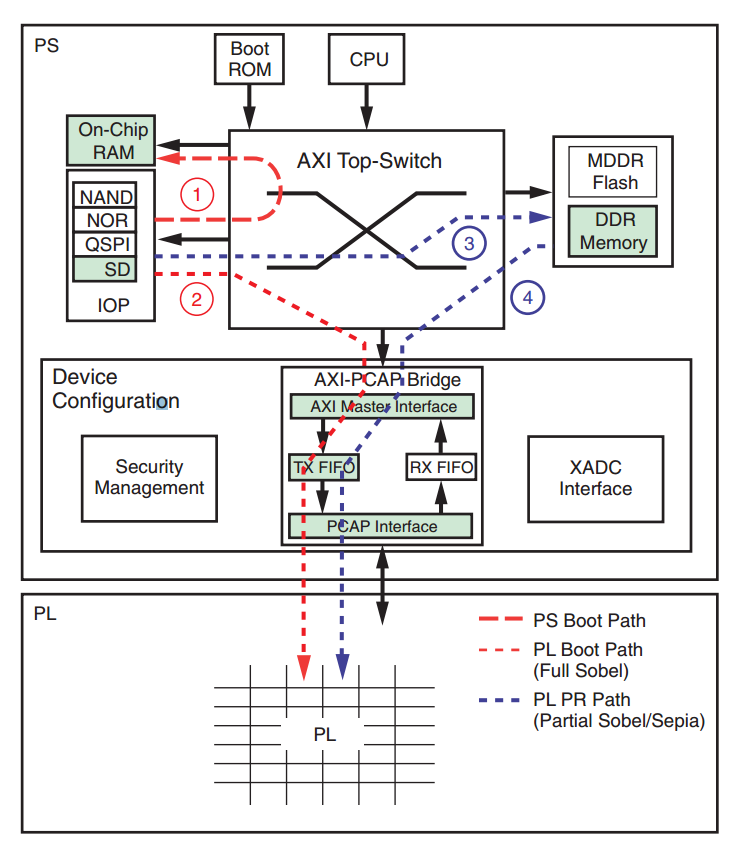
\includegraphics[scale=0.5]{protocollo_riconfigurazione.png}
\caption{Flusso di riconfigurazione}\label{fig:2}
\end{figure}

Il processo di reallocazione visto finora è riassumibile con la figura \ref{fig:2}, in cui si può vedere come la parte di  ``processing system'' (PS) configuri l'informazione da inviare alla parte di ``programmable logic'' (PL) tramite il bridge; caricato il file che rappresenta la nuova parte sintetizzata di programma dalla memoria, si invia alla parte da configurare PL utilizzando il protocollo del bridge.
Le aree precedentemente descritte quindi si trovano all'interno di PL, dove risiede l'effettiva parte logica. Queste aree normalmente possiedono una frammentazione interna ed esterna, in quando il codice non sempre occupa tutti i settori; proprio per questo si può deframmentare e ottenere dei settori vuoti in cui inserire runtime il codice.

Spostare un nuovo settore dentro la parte di logica programmata significa quindi configurare hardware precedentemente inattivo, dando quindi una nuova configurazione hardware e quindi un diverso comportamento del sistema. In base alla grandezza delle aree da spostare, possono coesistere all'interno dell'area PL, ma non avrebbe senso perché potrebbe significare avere hardware non utilizzato e configurato, quindi si spreca silicio.

\section{La progettazione}

Poichè non esiste un metodo standard per progettare, sviluppare o semplicemente simulare questi sistemi, si vuole creare un nuovo flusso di progettazione per gestire al meglio la fase di sviluppo. Poiché questi sistemi fanno parte di un sottoinsieme dei Sistemi Embedded generici, si utilizzerà ciò che è noto durante la fase di sviluppo di un normale Sistema Embedded per poi aggiungere ciò che serve per specializzare tale sistema in uno Metamorfico.

Il punto di partenza della progettazione non dovrà essere l'analisi dell'ambiente in cui calare il sistema da progettare, bensì sarà scindere cosa deve essere statico e cosa deve essere dinamico: una business logic, ad esempio, può essere una parte statica, mentre un insieme di range su cui fare misure può essere una parte dinamica perché dipende dall'ambiente. Una volta scelte le due parti, si procede con la progettazione come da prassi di un sistema embedded, progettando contemporaneamente queste parti: in questo modo, durante la progettazione, si può capire se le scelte adottate sono state corrette. Infine si configura l'hardware in modo da prepararlo per la sua futura metamorfosi, impostando la parte riconfigurabile, per poi osservare come cambia durante l'acquisizione delle informazioni.

Lo scopo di questa tesi sarà comunque capire come sviluppare al meglio la progettazione di questo tipo di sistema, comprendendo il grado di libertà che si può raggiungere per la parte dinamica e capire quale tipo di riconfigurabilità è più conveniente usare, oltre al fatto di essere sicuri che sia conveniente sfruttare la metamorfosi per risparmiare tempo e denaro durante la progettazione di un sistema embedded.

\chapter{Simulazione e sintesi di sistemi embedded}

Esistono vari metodi per progettare un sistema embedded; l'approccio ingegneristico più avanzato vuole che si progetti in maniera astratta il sistema, per poi calarlo in un contesto di descrizione tramite HDL per poi eseguire la sintesi.

\section{Simulazione}

Per la descrizione ad alto livello e simulazione, solitamente si utilizza SystemC a diversi livelli, passando da una descrizione mirata a osservare il comportamento dei diversi moduli durante la loro interazione (TLM), fino alla descrizione a livello di EFSM cycle accurate o analogica (RTL e AMS). I vantaggi dell'utilizzo di SystemC sono molteplici, soprattutto grazie allo scheduler interno si riesce a simulare correttamente i vari comportamenti a livello di segnali e attivazione dei moduli.

\section{Scheduler di SystemC}

Lo scheduler di SystemC è stato progettato in modo da rispettare una gerarchia di wakeup dei moduli, in quanto l'hardware solitamente è pilotato sia da un clock interno sia da segnali provenienti da diversi moduli, quindi è stato necessario modellare questo parallelismo tramite uno scheduler. Lo schedule eseguito dallo scheduler è diviso in passi:

\begin{enumerate}
\item Elaborazione: vengono create le strutture dati e viene fatto il binding delle porte;
\item Inizializzazione: vengono inizializzate porte e segnali e vengono fatti eseguire tutti i processi fino alla loro terminazione o al primo wait, in modo da creare una coda d'esecuzione iniziale;
\item Evaluation: viene fatto eseguire il primo processo pronto in coda d'esecuzione fino alla sua terminazione o ad un wait. Se vengono notificati eventi (con delle notify()), i processi interessati vengono messi in coda d'esecuzione. Se ci sono altri processi in coda pronti ad essere eseguiti ripeto le operazioni precedenti, altrimenti proseguo;
\item Update: vengono aggiornate porte e segnali ed aggiunti in coda d'esecuzione i processi sensibili ad essi;
\item Delta: vengono aggiunti alla coda d'esecuzione tutti i processi sensibili ad eventuali delta notification (notify(SC\_ZERO\_TIME)) Se ci sono altri processi in coda pronti ad essere eseguiti ripeto le operazioni precedenti a partire dalla fase di evaluation, altrimenti proseguo;
\item Timed: Vengono aggiunti alla coda d'esecuzione tutti i processi sensibili alla prima timed notification (notify(SC\_TIME(n,SC\_NS))). Aggiorno il tempo di simulazione (clock). Se ci sono altri processi in coda pronti ad essere eseguiti ripeto le operazioni precedenti a partire dalla fase di evaluation, altrimenti termino la simulazione.
\end{enumerate}

Grazie a questo scheduler, si ha uno strumento che simula correttamente un sistema embedded, rispettando anche i tempi accuratamente di esecuzione, osservabili tramite timestamp.

\section{Sintesi}

Una volta preparato il modello del sistema in SystemC e simulato correttamente, si procede con la descrizione hardware in HDL, simulazione ed infine sintesi. Solitamente si utilizza VHDL e Verilog, due linguaggi di descrizione hardware che permettono sia di simulare sia di sintetizzare. Solitamente se viene descritto correttamente il sistema in SystemC, il passaggio ad una descrizione HDL è quasi automatico, in quanto si rappresentano gli stessi concetti semanticamente; infatti questo processo dovrebbe essere una traduzione sintattica tra linguaggi.

\section{Simulazione e sintesi di sistemi metamorfici}

Poichè non esiste un metodo standard per progettare sistemi metamorfici, bisogna definire \textit{ex novo} un metodo efficace. Intuitivamente sarebbe consigliato utilizzare la stessa metodologia di progettazione di sistemi embedded standard, in modo da rendere facile l'apprendimento a chi è già abituato a progettare sistemi embedded consuetudinari, oltre a sfruttare le potenzialità di un metodo già assodato e verificato nel tempo.

\section{Simulazione con SystemC ReChannel}

Per la simulazione si vorrebbe utilizzare SystemC, in quanto offre una descrizione fedele dell'hardware da simulare e sfrutta la conoscenza di C++ per descrivere i sistemi. Attualmente esiste una libreria di SystemC per la descrizione di sistemi riconfigurabili chiamata ReChannel.

ReChannel è una libreria sviluppata dall'Università di Bonn dal Prof. Armin Felke nel 2008, ceduta a GreenSocs con licenza open-source l'anno successivo e attualmente non più mantenuta, a seguito degli aggiornamenti di SystemC 2.0 che non permettevano la compilazione. La libreria è stata aggiornata e riscritta durante la stesura di questa tesi ed ora è compilabile ed utilizzabile.

La libreria si basa sul concetto di \textbf{switch}, ovvero l'elemento cardine di un sistema riconfigurabile: deve esserci la possibilità di cambiare un modulo con un altro, possibilmente di stessa dimensione e con la stessa quantità di input e output. Lo switch, in questa libreria, viene rappresentato come una sorta di multiplexer, che tiene collegati i diversi moduli della parte riconfigurabile con il modulo della parte statica; al momento opportuno, deciso dal progettista, sia dinamicamente sia staticamente in fase di compilazione, si imposta in modo che attivi il canale di comunicazione tra il modulo attivato e la parte statica, mentre disattiva i moduli della parte dinamica che vengono sostituiti. Lo switch permette la comunicazione sia da parte statica a parte dinamica sia viceversa: la prima viene chiamata \textit{portal}, la seconda viene chiamata \textit{exportal}.

\begin{figure}[ht]
\centering
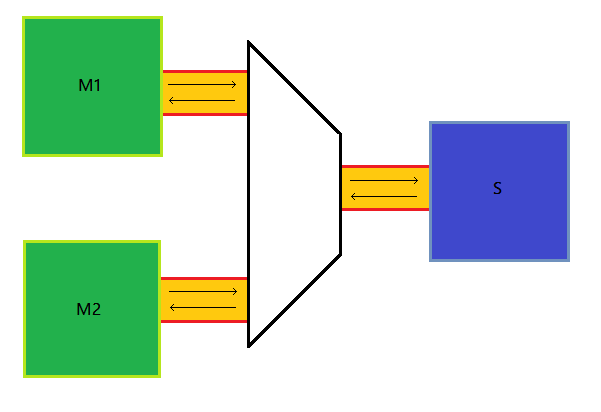
\includegraphics[scale=0.5]{portal.png}
\caption{Rappresentazione dello switch}\label{fig:3}
\end{figure}

Lo switch permette quindi la comunicazione tra i moduli della parte statica e della parte dinamica; la comunicazione può essere semplice (a un solo valore) o multivalore (coda fifo). Questo modella correttamente il concetto di bridge descritto precedentemente, ossia quel componente che permette la comunicazione tra le parti della FPGA. Questo si può vedere come una sorta di bus, che dirige il traffico point to point tra i diversi moduli.

L'utilizzo di questo componente per la comunicazione è un aspetto che si distanzia molto dalla solita progettazione di hardware in SystemC, poiché solitamente si definiscono i moduli con vari input e output e si effettua un collegamento punto-punto all'interno del main; con questa libreria invece si definiscono le modalità di comunicazione tra i moduli di diversa natura, per poi far gestire a questo componente i diversi collegamenti. Questo fatto modella correttamente le FPGA riconfigurabili moderne.

Il problema principale ora, conoscendo lo scheduler di SystemC, è gestire le modalità di schedule dei moduli della parte riconfigurabile; è necessario quindi estendere lo scheduler nativo con delle nuove opzioni.

\begin{figure}[ht]
\centering
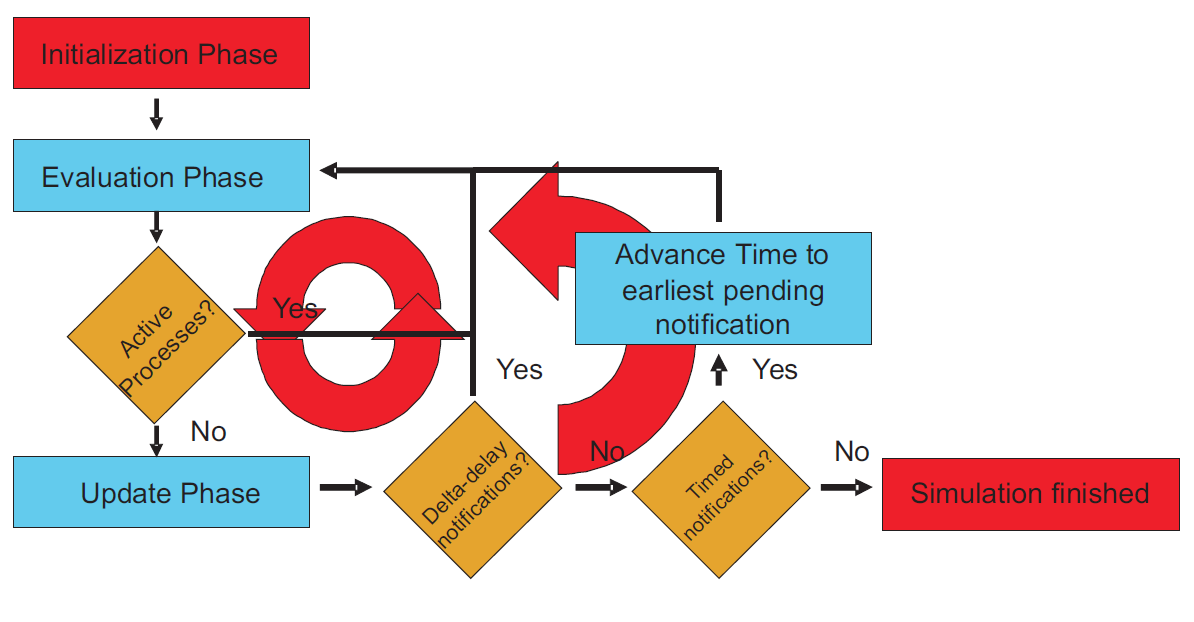
\includegraphics[scale=0.5]{scheduler_rechannel.png}
\caption{Scheduler esteso con ReChannel}\label{fig:4}
\end{figure}

Come si può notare con la figura \ref{fig:4}, è stato esteso lo scheduler dando priorità alla riconfigurazione, quindi nella fase di Evaluation si aggiunge un'ulteriore fase, ovvero il controllo sui processi attivi, oltre ad aggiungere passaggi nella fase di inizializzazione.
Durante la fase di inizializzazione, vengono istanziati tutti i moduli riconfigurabili e disattivati; è compito del progettista decidere quale modulo inizialmente deve essere attivato, ma non è necessario che ci siano moduli attivi. Successivamente, un modulo può essere attivato in qualunque momento; lo scheduler lo attiverà appena entrerà nella parte finale della fase di Evaluation, controllando che ci siano processi attivi pendenti (quindi da attivare).

Solitamente si utilizza un modulo statico che si occupa di fare da transattore tra la parte statica e la parte dinamica; solitamente viene chiamato processo ``Top'' e si occupa sia di descrivere lo switch sia di effettuare la commutazione dei moduli della parte dinamica. Anche in questo caso, viene modellata correttamente l'architettura riconfigurabile, in quando deve esserci un'entità del sistema che si occupa di effettuare la riconfigurazione, che può essere il processore nella board della FPGA o lo stesso progettista se si descrive una riconfigurazione statica.

Un ultimo aspetto molto importante che simula correttamente la realtà è la possibilità di impostare il tempo necessario per la riconfigurazione: ogni modulo, in base alla FPGA target, può metterci tempi differenti per essere attivato e disattivare gli altri, quindi è neccesario un meccanismo per modellare il tempo di riconfigurazione. Questa libreria modella il tempo di riconfigurazione in base al caso pessimo di tempistiche, ovvero permette al progettista di impostare il tempo massimo che impiega il modulo ad essere attivato (infatti non sempre impiega lo stesso tempo per essere riconfigurato, per questo bisogna ragionare per caso pessimo). Può essere deciso questo tempo secondo le specifiche della FPGA target proporzionali all'area che il circuito ricopre (si possono effettuare delle stime in base a quante e quali operazioni vengono eseguite).


\section{Sintesi}

La sintesi di questi sistemi è molto simile alla sintesi dei normali sistemi embedded, poiché si utilizza HDL compilato e sintetizzato tramite tool automatici.

La traduzione da SystemC Rechannel a VHDL è molto semplice: si rappresentano i diversi moduli come moduli statici, contrassegnando i moduli dinamici con un nome riconoscibile ed incrementale (es: reconfigurable\_module1, reconfigurable\_module2, ecc...), ci si assicura che tutto sia stato scritto correttamente e si importano i file nel programma di sintesi prescelto.

Solitamente i programmi di sintesi vengono offerti direttamente dai produttori della FPGA target (ad esempio per la Virtex 4 danno in dotazione il programma) e permettono di impostare facilmente i diversi moduli scritti in HDL tramite interfaccia grafica. Tutti i tool automatici partono quindi dalla descrizione in HDL e, tramite un'ulteriore sforzo del progettista nell'impostare il comportamento dei moduli, acquisiscono la particolarità di essere statici o dinamici.

\begin{figure}[ht]
\centering
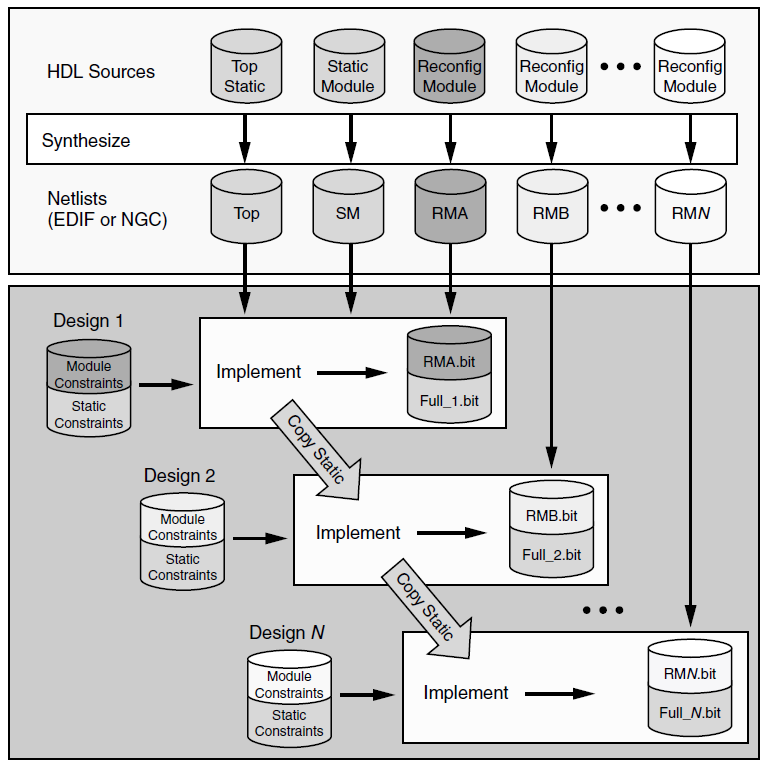
\includegraphics[scale=0.6]{processo_sintesi.png}
\caption{Processo di sintesi eseguito da un tool automatico}\label{fig:5}
\end{figure}

Come si può notare con la figura \ref{fig:5}, il tool automatico identifica i sorgenti come moduli che devono essere sintetizzati; possiamo notare i diversi insiemi di moduli tra cui il modulo ``Top'', già visto precedentemente con SystemC ReChannel, che identifica il transattore tra la parte statica e la parte dinamica del sistema. Una volta sintetizzati i sorgenti, si crea una Netlist, ovvero si creano i collegamenti interni ed esterni tra moduli, in modo da definire il metodo di comunicazione. Fatto ciò, il tool identifica in automatico tutti i differenti design che si creeranno durante il ciclo di vita del sistema, in base alle configurazioni possibili definite nella Netlist; ogni Design è una copia statica presente in memoria, quindi una volta sintetizzata esistono le configurazioni in memoria già pronte per essere nuovamente sintetizzate in hardware (solitamente risiedono nella memoria Flash).

L'ultimo passaggio del tool automatico è la creazione delle partizioni della FPGA, perché deve essere possibile identificare dove caricare la parte riconfigurabile e dove deve rimanere staticamente il codice; viene creato quindi il file delle partizioni, solitamente chiamato \textit{XPARTITION.xml}, che risiede in memoria e viene consultato ogni volta che deve avvenire una riconfigurazione.

\chapter{Metodologia di progettazione proposta}

Lo scopo di questo documento è di proporre una metodologia efficiente di progettazione e simulazione per questa particolare architettura. Attualmente non esiste un metodo standard per la progettazione di sistemi basati su questa architettura, quindi si è cercato di proporre un metodo più efficiente possibile per garantire anche a chi non conosce approfonditamente questa tecnologia di poterla sfruttare al meglio.
Per decidere uno stile di progettazione, si è deciso di basarsi su uno stile già noto nei sistemi consuetudinari embedded, ovvero la progettazione di macchine a stati finiti. La tecnica delle macchine a stati finiti garantisce chiarezza di progettazione e un flusso chiaro di istruzioni che vengono eseguite durante la ``vita'' del sistema, evidenziando anche i possibili blocchi ed anomalie che possono esserci durante l'esecuzione. Inoltre ci si è serviti del noto concetto di ``macchine a stati finiti non deterministiche'': è possibile rappresentare un sistema a stati che può comportarsi ``contemporaneamente'' in molteplici modi, quindi avere più comportamenti tramite lo stesso input in ingresso (solitamente evitato durante la progettazione delle macchine a stati finiti, in quanto non è implementabile).

La progettazione proposta quindi si differenzia in diverse fasi:

\begin{itemize}
  \item \textit{analisi del sistema}, evidenziando cosa potrebbe essere trattato come sistema standard e sistema riconfigurabile; si analizza quindi cosa deve rimanere statico per tutta l'esecuzione di un algoritmo e cosa può cambiare durante l'esecuzione;
  \item \textit{analisi degli stati}, ovvero si comincia a creare il sistema a stati evidenziando come evolve il sistema dinamico dividendolo in fasi; si deve quindi creare una macchina a stati generale creando il flusso di esecuzione del sistema, ma non rappresentando ciò che succede all'interno degli stati (perché si suppone che per diverse configurazioni ci saranno diversi comportamenti all'interno delle suddette fasi);
  \item \textit{definizione degli stati}, ovvero si ``disegnano'' gli stati del sistema riconfigurabile, evidenziando le diverse macchine a stati che vengono prodotte: in questa fase si devono ottenere più macchine a stati duplicate, con lo stesso numero di stati il cui contenuto però cambia tra macchine, perché il flusso di esecuzione sarà lo stesso ma ciò che avviene negli stati deve essere differente;
  \item \textit{definizione del Top}, il componente che deve guidare lo svolgimento delle attività della parte riconfigurabile; questo deve avere anch'esso la stessa macchina a stati dei moduli riconfigurabili, ma sarà l'unico componente che può decidere in quale stato deve trovarsi il sistema;
  \item \textit{implementazione e simulazione}, tramite il tool SystemC Rechannel;
  \item \textit{validazione e sintesi}.
\end{itemize}

\begin{figure}[!ht]
\centering
\includegraphics[scale=0.6]{reconfigurable_structure.png}
\caption{Struttura finale del sistema progettato}\label{fig:6}
\end{figure}

Il sistema finale dovrebbe essere simile alla figura \ref{fig:6}: si può notare che il sistema risulta modulare e ben diviso tra parte statica e parte dinamica: questo, oltre a facilitare la comprensibilità del progetto, garantisce anche una buona analisi in fase di simulazione e validazione, in quanto è possibile analizzare nel dettaglio le singole parti del sistema e garantire l'analisi di ogni stato e di ogni modulo.
La divisione netta tra parte statica e parte dinamica garantisce anche il parallelismo di esecuzione tra le diverse parti del sistema: potenzialmente la parte statica può eseguire codice in maniera del tutto asincrona rispetto alla parte dinamica, garantendo quindi più potenza di calcolo in termini di velocità. Infine, rappresentare il sistema con macchine a stati finiti permette di effettuare tutte le ottimizzazioni note per diminuire il numero degli stati del sistema, guadagnando ancor più spazio.
Si vedrà nel dettaglio con il caso di studio il guadagno ottenuto da questa architettura proposta in contesto di vincoli realtime hard.

Se da un lato si hanno degli ottimi benefici, con questa configurazione si ottengono anche degli svantaggi dal punto di vista implementativo: la parte dinamica e la parte statica necessitano di comunicazione tramite il bus, però essendo entrambi asincroni necessitano di meccanismi di sincronizzazione per evitare di perdere dati. Inoltre, visto che questo tipo di sistemi viene calato in contesti critici, essendo sistemi embedded, bisogna essere sicuri di progettare il sistema in modo che non presenti anomalie e quindi perdere l'efficacia dell'utilizzo di questa architettura.
È quindi necessario garantire che il sistema sia sempre in stato ``safe'': come tutti i sistemi asincroni, se sono presenti le 3 condizioni necessarie (mutua esclusione, hold and wait, no preemption, attesa circolare), il sistema può andare in deadlock, quindi è necessario adottare tutte le strategie necessarie per evitare ciò.
Fino ad ora la garanzia di stato safe del sistema dal punto di vista di asincronicità era lasciata al progettista, con questo progetto si propone invece un tool automatico per generare il software per SystemC Rechannel adottando questo metodo di progettazione, in modo da lasciare al progettista solo il compito di pensare e progettare il comportamento dei moduli del sistema.

Con questo progetto quindi non si propone esclusivamente una metodologia di progettazione, ma anche un tool automatico per progettare correttamente questi sistemi.


\section{Rappresentazione della metodologia di progettazione}

Il processo di progettazione proposto per questi sistemi deve seguire il Sequence Diagram proposto nella figura \ref{fig:7}.

\begin{figure}[!hb]
\centering
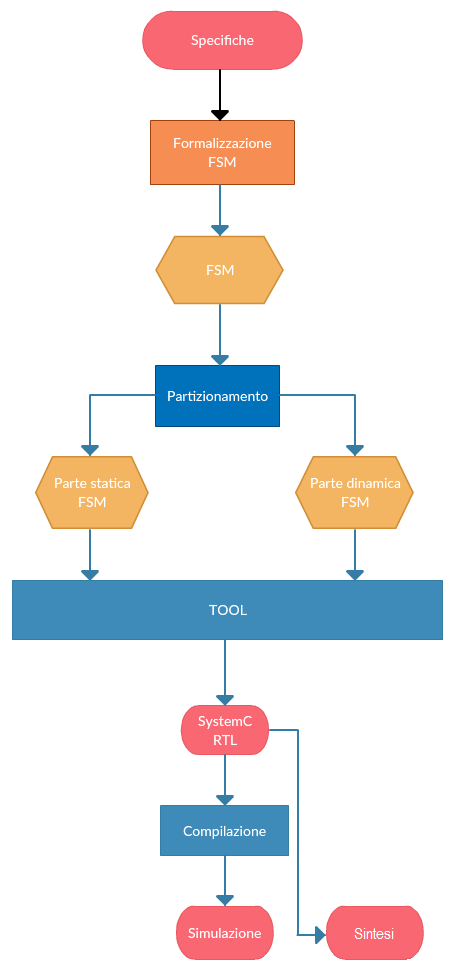
\includegraphics[scale=0.75]{processo.png}
\caption{Sequence diagram del processo di progettazione}\label{fig:7}
\end{figure}

Si può notare che il processo proposto risulta lineare, senza cicli e con un'unica diramazione: questo è molto importante dal punto di vista dello sviluppo in quanto non costringe lo sviluppatore ad eseguire delle scelte in base alla situazione e non deve iterare varie parti della progettazione in base al tipo di progetto. La complessità di progettazione quindi è pressochè costante, mentre il punto critico della diramazione consiste in un singolo passo quindi non può portare problemi di sviluppo (dal punto di vista di tempistiche e di utilizzo di risorse).

Tutto parte dalla comprensione delle specifiche da parte del progettista: queste, descritte in qualsiasi forma, devono essere ben comprese dal progettista per identificare la ''forma'' del sistema futuro. Ogni sistema può essere rappresentato con una macchina a stati finiti estesa, quindi è necessario che il progettista riesca ad indentificare come formalizzare il sistema tramite una FSM estesa. Una volta formalizzata la FSM estesa, si può descrivere l'intero sistema disegnandolo come fosse una FSM.

La FSM può essere descritta a proprio piacimento, ma deve essere abbastanza eloquente in modo da far capire quali siano le parte predestinate alla riconfigurazione. Questo significa che ogni parte del sistema deve essere descritta in maniera generica, tralasciando gli aspetti implementativi (ovvero la descrizione di ciò che avviene all'interno degli stati del sistema), ma bisogna descrivere nel dettaglio ogni potenziale stato del sistema. 

Una volta ottenuta la FSM del sistema, si esegue manualmente il partizionamento della FSM candidata alla parte statica del sistema e alla parte dinamica: per farlo si possono seguire le seguenti euristiche:

\begin{itemize}

\item considerare le parti ripetute della FSM (dal punto di vista semantico): quando si nota che una parte della FSM viene ripetuta, ovvero ha le stesse transizioni nel grafo e il comportamento interno ha lo stesso significato (ma l'implementazione futura genererà un comportamento diverso), allora si può inserire quella parte di FSM nella parte dinamica futura della FSM, mentre il restante grafico si implementerà nella parte statica;

 \item identificare i potenziali punti in cui il sistema dovrebbe riconfigurarsi e cambiare comportamento (rimanendo semanticamente uguale tra le configurazioni): in alcune situazioni è ben chiaro quando il sistema deve cambiare la propria descrizione interna in base alla situazione ed eseguire un task che contiene delle piccole variazioni rispetto ad altri. 

\end{itemize}

Quindi si può capire che ciò che caratterizza la parte dinamica del sistema è la semantica: devono essere implementati comportamenti diversi, ma la semantica del task deve essere la medesima per ogni riconfigurazione. Basti pensare un forno con diverse modalità di cottura, ognuna ha il significato di ``cuocere qualcosa'', ma la modalità di cottura è differente, quindi il codice che implementa la cottura sarà differente.

~ 

\begin{figure}[!ht]
\centering
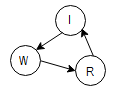
\includegraphics[scale=1.5]{fsm.png}
\caption{Descrizione della FSM standardizzata}\label{fig:8}
\end{figure}

In aggiunta a ciò, si propone anche uno standard di FSM presentato nella figura \ref{fig:8}: poiché questo metodo di progettazione è molto efficiente, si può utilizzare uno standard anche di rappresentazione della macchina a stati, in modo da rendere più semplice e chiara la partizione tra sistemi e più semplice la descrizione degli stati.

Questa FSM è composta da almeno 3 stati, uno di questi può essere esteso a quanti stati si vuole. Lo stato iniziale è lo stato ``Init'' (nella figura, ``I''), in cui avviene l'inizializzazione del sistema riconfigurabile (quindi si resettano i valori delle variabili, si aspetta che la configurazione sia pronta e si prepara il sistema ad eseguire il futuro algoritmo); lo stato successivo è lo stato di ``Work'' (nella figura, ``W''), in cui si esegue effettivamente l'algoritmo per cui il sistema è stato progettato; questo stato può essere esteso a quanti stati si vuole, in base al modello di sistema che si è rappresentato precedentemente. Infine, lo stato ``Reconfigure'' (nella figura, ``R''), esegue la riconfigurazione del sistema per ottenere un comportamento diverso dal precedente; si può dire che questo stato è l'opposto della fase di Init, in quando prepara il sistema alla futura fase di Init di un'altra configurazione.

Non è necessario rappresentare la FSM nel modo precedentemente descritto, ma è consigliato in quanto aiuta a comprendere meglio la partizione del sistema e a creare gli stati correttamente ed in maniera ordinata.

~ 

Una volta eseguito il partizionamento si può ottenere il codice del sistema finale in 2 modi: o scrivendo il codice a mano in SystemC Rechannel, o utilizzando un tool automatico che genera il codice SystemC partendo da una descrizione ad alto livello. Il tool automatico verrà descritto nella prossima sezione.

Infine, avendo il codice SystemC, è possibile sia simulare il sistema, tramite compilazione, sia generale l'effettivo codice finale per eseguire il deploy su FPGA dedicata. Per convertire il codice da SystemC a Netlist, si può utilizzare un qualsiasi tool automatico di conversione da codice a Netlist.

\section{Tool automatico (Pyngu)}


\begin{figure}[!ht]
\centering

\includegraphics[scale=0.2]{pyngulogo.png}
\caption{Logo del tool Pyngu}\label{fig:9}
\end{figure}


Poichè il processo di generazione di codice è standard e meccanico, è possibile implementare con un tool automatico tutto il processo di scrittura di codice utilizzando un programma di supporto che possa aiutare il progettista. 

Poiché non tutti i progettisti di sistemi embedded conoscono la teoria e la parte implementativa dell'hardware riconfigurabile, è utile astrarre il più possibile dall'utilizzo di SystemC Rechannel e dallo studio dei sistemi riconfigurabili e concentrarsi sulla semantica del sistema. Nasce quindi la necessità di rendere disponibile al progettista un tool automatico che utilizza un mezzo semplificato per descrivere ed implementare il sistema, senza perdere comunque l'espressività di SystemC Rechannel. Utilizzando questo tool, si implementa, secondo lo standard proposto precedentemente, l'intero sistema finale, ottenendo il codice SystemC Rechannel senza sapere i dettagli implementativi della libreria.

Il tool proposto si chiama Pyngu, un interprete e compilatore code-to-code scritto in Python; il nome deriva dal noto personaggio dei cartoni, Pingu, che parlava una lingua incomprensibile all'uomo ma riusciva a farsi capire dai suoi simili, oltre al fatto di capire il linguaggio umano (ciò che fa anche questo tool, ovvero trasforma una descrizione ad alto livello del sistema in un linguaggio che non sempre è noto al progettista); l'aggiunga del suffisso ``Py'' è dovuto allo standard Python dei progetti.

Il tool prende in input una descrizione ad alto livello del sistema completo, tenendo conto della divisione tra parte statica e parte dinamica: in questo modo, il tool genererà i differenti file in base al modo in cui è stato descritto il sistema, tenendo separata la parte statica dalla parte dinamica.

Come linguaggio di base ad alto livello è stato scelto YAML (pronunciato `jaemel), un linguaggio di serializzazione dati che permette facilmente di descrivere con item e sequenze dati e parti di codice; \'{E} stato scelto questo linguaggio perché è molto semplice da imparare e non richiede nessuna conoscenza di programmazione, in modo da renderlo comprensibile anche a chi non conosce i sistemi riconfigurabili.

Seguendo le regole del linguaggio di base ed aggiungendo delle parole chiave che hanno significato solo per il tool automatico, il tool automatico genera il sistema descritto. In particolare, il tool esegue gli stessi passi che esegue il progettista mentre progetta il sistema: identifica la descrizione della parte statica e dinamica del sistema, trasforma la descrizione in FSM in SystemC e infine genera il codice del sistema finale.

Il tool fa sia da interprete sia da compilatore code-to-code: prima di tutto controlla che non ci siano errori nel codice scritto dal progettista, analizzando i tag che riesce a riconoscere, poi, partendo da dei template di file SystemC che contengono la struttura del sistema secondo lo standard, popola i file finali SystemC trasformando ciò che ha descritto il progettista in codice.

Inoltre il tool rispetta lo standard di SystemC Rechannel, aggiungendo lo standard proposto in questa tesi, oltre al fatto di gestire le condizioni di safety descritte precedentemente: utilizzando correttamente questo tool e il relativo linguaggio, si eviteranno futuri errori di implementazione che potrebbero compromettere l'intero funzionamento del sistema.

\subsection{Il linguaggio (PynguLang)}

Il linguaggio riconosciuto dal tool automatico serve per descrivere sia la parte statica sia la parte dinamica del sistema ad alto livello basandosi sulla conoscenza dello standard YAML. Il progettista dovrà essere in grado, dopo lo studio di questo linguaggio, di creare un file ``.yaml'' contenente la descrizione del sistema secondo lo standard del linguaggio, in modo da astrarsi completamente dalla conoscenza e studio di SystemC Rechannel.

La descrizione del sistema tramite il linguaggio  consiste in 2 passaggi: la descrizione della parte di struttura delle singole parti del sistema (quindi parte statica e parte dinamica) e la descrizione del comportamento interno delle singole parti.

~ 

La prima parte consiste nel descrivere le porte di ingresso, le uscite, le variabili interne e i tipi di segnali che compongono le parti del sistema. Le parole chiave sono contraddistinte dalla presenza della stringa ``\textit{init}''

\begin{figure}[!ht]
\centering
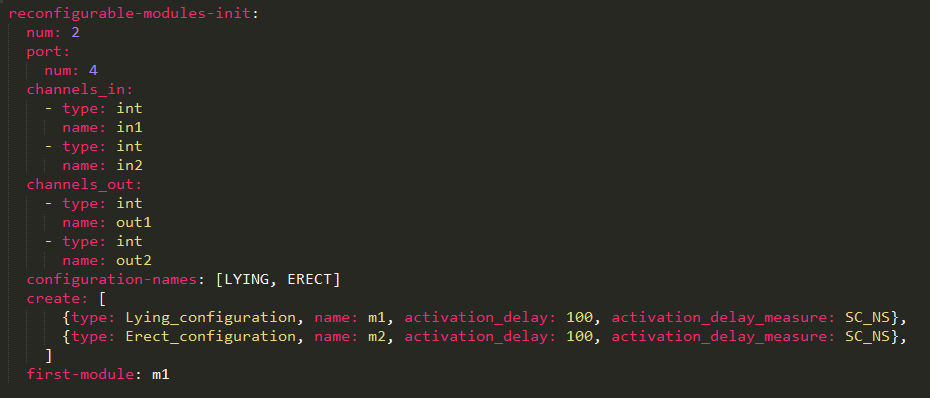
\includegraphics[scale=0.6]{pyngu_init_example.png}
\caption{Esempio della prima parte della descrizione del sistema}\label{fig:10}
\end{figure}

In questa parte, si possono descrivere: 
\begin{itemize}

\item il Top, ovvero la parte statica del sistema (tramite il tag ``top-init''), di cui si possono definire le variabili (``variables''), i canali di input e output (``channels'') e i canali di comunicazione con la parte dinamica (``portals'') ;

\item i moduli riconfigurabili (tramite il tag ``reconfigurable-modules-init''), di cui si possono definire la quantità di moduli che il sistema può avere (``num''), il numero di porte di ingresso e uscita che può avere (``port->num''), il tipo di canali di comunicazione che può avere (``channels\_in'' e ``channels\_out''), il nome che si vuole dare alle diverse configurazioni (``configuration\_names''), il primo modulo che deve attivarsi e le modalità di caricamento dei moduli (``create'', con cui si può definire il tempo di attivazione tramite ``activation\_delay'' e l'unità di misura in cui viene espresso questo tempo tramite ``activation\_delay\_measure'');

\item la FSM in comune tra i due sistemi (tramite il tag ``fsm-init''), di cui si definiscono il numero di stati (``num''), e il nome degli stati (``states'');

\item altre variabili di supporto definite dal progettista (tramite il tag ``common-other-variables''), di cui si identifica il tipo (tramite ``type''),  il nome (tramite ``name'') e il relativo valore se necessario (tramite ``value'');

\end{itemize}

Nella prima parte quindi si dà particolare enfasi alla parte di specifiche strutturali, dove è fondamentale capire gli inputs e gli outputs del sistema, oltre ad implementare il metodo corretto di comunicazione tra parte statica e parte dinamica del sistema.

~ 

La seconda parte invece consiste nello scrivere l'effettivo codice che verrà eseguito all'interno dei diversi sistemi. . Le parole chiave sono contraddistinte dalla presenza della stringa ``\textit{code}'' e il linguaggio permette l'inserimento di codice puro (raw) di SystemC.

\section{Utilizzo del tool durante la progettazione}

Il tool automatico risulta essere particolarmente efficace durante la progettazione, avendo fatto le giuste scelte implementative seguendo il flusso proposto. In particolare, il linguaggio riconosciuto dal tool, basato appunto su YAML, ha massimo potere espressivo nel contesto del flusso di progettazione, in quanto permette di descrivere ogni componente del sistema riconfigurabile da produrre. Se sono state fatte le scelte giuste (precedentemente descritte), la conversione delle FSM ottenute sarà molto facile seguendo il linguaggio, mentre scelte sbagliate renderanno la descrizione tramite il linguaggio leggermente più complesse (o comunque non efficaci).

Il tool inoltre non ha un ruolo fondamentale, semplicemente aiuta il progettista che non conosce la libreria oppure necessita di una scrittura velocizzata del codice: lo stesso codice SystemC ottenuto dal tool può essere scritto a mano dal progettista. Si suppone che comunque il tempo necessario per apprendere il linguaggio PynguLang sia molto minore rispetto ad apprendere il funzionamento della libreria SystemC Rechannel, quindi un guadagno di apprendimento si ha, oltre al fatto di ottenere codice che risulta essere safe e corretto per costruzione.



\chapter{Caso di studio}

Per verificare le potenzialità di questa architettura e del metodo di progettazione proposto, è stato implementato un progetto complesso che comprende molteplici aspetti avanzati dell'applicazione dell'informatica; in questo modo, si è proposto un esempio robusto per far notare i pregi (anche dal punto di vista della complessità di progettazione) di questa architettura.
Il caso di studio consiste in un robot \textit{intelligente} e \textit{riconfigurabile} che deve essere in grado di affrontare un percorso ad ostacoli per raggiungere una fonte di calore, quindi calato in un contesto di robot di salvataggio che è in grado di ricercare persone in ambienti avversi o identificare fonti di incendi e tentare di domare le fiamme. Il tutto è stato implementato con diversi tool di simulazione che sono stati fatti comunicare e rispettando i vincoli temporali di un sistema reale (quindi utilizzando clock, tempi fisici realistici con tutti i problemi di hard realtime annessi).
Sono stati utilizzati quindi i seguenti tool di simulazione:

\begin{itemize}
  \item \textit{Blender} per la progettazione e implementazione della parte fisica ed estetica del robot;
  \item \textit{V-REP} per la simulazione del robot implementato in Blender, utilizzando il più possibile una fisica realistica;
  \item \textit{SystemC Rechannel} per la simulazione dell'hardware riconfigurabile;
  \item \textit{Linux Ubuntu} per simulare il programma di intelligenza artificiale che dovrebbe essere eseguito su un qualsiasi processore e che deve interfacciarsi con la parte riconfigurabile (implementata in SystemC Rechannel).
\end{itemize}

Il funzionamento del sistema è il seguente: il robot può avere 2 differenti configurazioni, ovvero configurazione a quadrupede e configurazione a doppio serpente; queste configurazioni vengono pilotate e mosse dal sistema riconfigurabile in base al percorso che il robot deve eseguire. Il robot è sensibile alle fonti di calore, ovvero tramite sensore di visione di calore, è in grado di percepire dove si trova una fonte di calore e capire quanto è distante da esso. Per capire quanto è distante dalla fonte di calore, viene fatto uno studio statistico sulla quantità di pixel rossi che appaiono nell'immagine acquisita.
Il robot non conosce l'ambiente in cui si trova, si deve solo basare sui sensori di distanza posti su di esso, uno per ogni lato, e sul sensore di visione; non deve interagire con l'ambiente ma deve solo essere in grado di non essere ostacolato nei suoi movimenti. Il task del robot consiste nel raggiungere o di avvicinarsi il più possibile alla zona di calore e, per farlo, deve riuscire a trovare il percorso migliore (ovvero quello fattibile).
La strategia del robot consiste nel ``provare'' quale delle 2 sue configurazioni può essergli utile per raggiungere l'obbiettivo: durante il suo tragitto, potrebbe trovare un ostacolo che gli impedisce di proseguire, quindi deve essere in grado di oltrepassarlo o passandoci sotto oppure raggirandolo. Deve inoltre essere in grado di capire se la scelta di strategia per oltrepassare l'ostacolo è corretta: è ammesso che il robot esegua degli sbagli durante le sue scelte, in quanto non ha una mappatura dell'ambiente, ma deve essere in grado di tornare indietro nelle sue scelte, capire quando è avvenuto l'errore della sua scelta e quindi adottare una strategia diversa per raggiungere il target.
La scelta del tragitto viene sempre attuata in base a dove si trova la fonte di calore: l'euristica è appunto quella di minimizzare il tragitto andando in direzione sempre dove la concentrazione di pixel rossi è maggiore. Ovviamente in questo modo il robot non sa dove si trovano gli ostacoli in quanto è in grado di ``vedere'' soltanto le fonti di calore, quindi il suo tragitto sarà pieno di scelte.

A causa della difficoltà reale del progetto, sono state fatte diverse assunzioni:
\begin{itemize}
  \item il terreno di simulazione è liscio e piatto;
  \item gli ostacoli sono semplici e facilmente individuabili dai sensori del robot (quindi composti da figure solide semplici);
  \item l'ambiente risulta statico, quindi non ci sono ulteriori interazioni col robot;
  \item i movimenti del robot sono rettilinei, a meno di problemi dovuti alla progettazione manuale del robot (giunti non perfettamente allineati, misure approssimative, errori del simulatore).
\end{itemize}

Si vedranno ora nel dettaglio le diverse implementazioni dei componenti.

\section{Hardware riconfigurabile}

Il sistema riconfigurabile svolge la funzione di moto, riconfigurazione e sensoristica del robot: tutta la parte di cinematica viene delegata a questa parte, con i relativi controlli sui sensori. Si potrebbe paragonare ad un sistema nervoso adattivo: esso è in grado di adattarsi all'ambiente percependolo, ma non comprendendolo. La comprensione di tutti i segnali viene delegata alla parte di intelligenza artificiale, questa parte si occupa solo di acquisire dati e di inviarli al ``sistema di controllo e comprensione''.
Questo è stato implementato in simulazione su SystemC Rechannel ed è composto da 2 entità:

\begin{itemize}
  \item \textit{Top}, che contiene la parte di controllo del sistema riconfigurabile che si interfaccia direttamente con i moduli riconfigurabili; è in grado di dare il comando di riconfigurazione ai moduli riconfigurabili e di acquisire i segnali dai sensori del robot per trasformarli in dati comprensibili alla parte di intelligenza;
  \item \textit{Moules}, che contiene i moduli riconfigurabili che eseguono gli algoritmi di movimento.
\end{itemize}

L'algoritmo di funzionamento è il seguente: il Top controlla i sensori del robot e li invia al sistema di intelligenza artificiale che li elabora; successivamente il Top riceve il comando in base ai valori dei sensori e il Top, in base alla sua macchina a stati, invia l'azione da eseguire al modulo riconfigurabile attualmente attivo.
Parallelamente il Top controlla se deve essere eseguita una riconfigurazione: se deve essere riconfigurato il sistema, dealloca il modulo riconfigurabile e attiva quello prescelto, in modo che venga eseguita la prossima azione su quel modulo.
Contemporaneamente il modulo riconfigurabile attualmente attivo esegue l'azione che gli è stata precedentemente inviata dal Top, per poi attendere il prossimo comando.

Il Top è composto quindi dai seguenti componenti:

\begin{itemize}
  \item \textit{activator}, che si occupa di attivare e deattivare i moduli riconfigurabili;
  \item \textit{producer}, che invia i dati ai moduli riconfigurabili;
  \item \textit{controller}, che si occupa di tenere traccia della riconfigurazione attuale e di quella futura;
  \item \textit{monitor}, che si occupa di leggere i dati di risposta dei moduli riconfigurabili.
\end{itemize}

Si ha quindi anche parallelismo interno al modulo Top, in quanto deve essere in grado di gestire contemporaneamente i diversi aspetti della riconfigurazione. Questo parallelismo è gestito da SystemC Rechannel, però lo scambio di messaggi (che risulta bloccante secondo l'architettura Client-Server rispettivamente dei moduli riconfigurabili e del Top) viene gestito dal progettista.

\section{Robot riconfigurabile}

È stato creato un robot riconfigurabile, ovvero capace di mutare la propria forma in modo da presentare una cinematica differente per ogni riconfigurazione. La caratteristica principale di questi robot è di essere composti da moduli semplici che, uniti tra loro, creano una struttura più complessa.


\subsection{I robot riconfigurabili}

\begin{figure}[htbp]
\centering
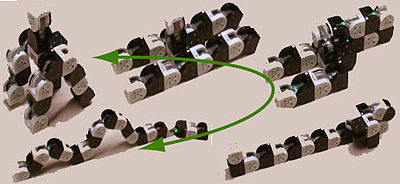
\includegraphics[scale=0.5]{robot_riconfigurabile1.jpg}
\caption{Un robot riconfigurabile (M-TRAN III)}\label{fig:9}
\end{figure}

I robot riconfigurabili sono macchine con cinematica autonoma che possiedono una morfologia variabile. Con morfologia variabile si intende la capacità di mutare forma e quindi la configurazione dei giunti, in modo da permettere al robot di compiere movimenti diversi, quindi avere una cinematica diversa. La caratteristica principale di questi sistemi è quindi di riarrangiare la connessione tra le parti in base a determinate circostanze, in modo da eseguire diversi task, per tornare in situazioni safe, o per ripararsi.
Questi si dicono anche ``robot modulari'' in quanto sono composti da piccoli componenti (moduli) che si riassemblano tra loro e creano il robot nella sua completezza.

Questi sistemi uniscono diversi aspetti della robotica e di altre discipline, come la progettazione di sistemi embedded, le reti di sistemi embedded e l'intelligenza artificiale, poiché questi sistemi hanno bisogno di una visione completa del mondo circostante ma soprattutto dei pezzi di cui sono composti.

Un robot riconfigurabile è composto da un insieme omogeneo di moduli, che sono tutti simili di forma e di cinematica tra loro (solitamente con 1 grado di libertà) che sono in grado di comunicare e ``organizzarsi'', ovvero coordinarsi per collaborare. La collaborazione serve ai moduli per ``capire'' come collegarsi tra loro e creare una struttura differente per ogni situazione.

Esistono differenti tipi di robot riconfigurabili, tutti raggruppati in 2 macro aree:
\begin{itemize}
  \item \textit{parzialmente riconfigurabili}, che sono composti da moduli precedentemente assemblati che, con delle forme prestabilite si riconfigurano in modo da cambiare la morfologia del robot (come in questo caso di studio);
  \item \textit{completamente riconfigurabili}, che non hanno una forma prestabilita e tutti i moduli sono inizialmente separati, per poi comporsi tra loro completamente in base alla situazione.
\end{itemize}

Questo stile di progettazione del robot porta essenzialmente vantaggi funzionali e vantaggi economici: i primi sono dovuti alla potenziale robustezza e adattabilità del robot rispetto all'ambiente, rispetto ai robot convenzionali; i secondi derivano dal fatto di costi di produzione ridotti (si creano moduli tutti uguali in serie) e costi di progettazione sia hardware sia software ridotti (si progetta un singolo modulo e si crea un software di coordinazione che è valido per ogni modulo).

Questi robot non sono ancora diventati effettivamente utilizzati in quanto presentano degli svantaggi logistici piuttosto importanti: oltre al fatto che sono ancora in fase sperimentale, non vengono ancora sfruttati metodi ingegneristici per la progettazione, in particolare non è ancora stata studiata una tipologia di hardware e software che, accoppiati, potessero massimizzare le performance e potessero minimizzare i consumi, oltre al fatto che non esiste un modo coerente e standard per simulare e quindi testare il sistema completo.
Il problema principale infatti di quando si progetta il robot è avere una rappresentazione abbastanza corretta e simile alla realtà, in modo da passare alla fase di produzione per il test reale in maniera piuttosto trasparente ed efficace (minimizzando quindi i costi di progettazione e produzione).

Un aspetto teorico legato a questi robot è la modellazione simile a quella che si utilizza quando si progetta un nuovo linguaggio. Questa infatti è stata formalizzata con aspetti di di analisi ``sintattica'' e ``semantica'': poiché sono strutture difficili da studiare, il moto di questi robot viene studiato attraverso la definizione di un linguaggio, quindi definendo la relativa grammatica (movimenti base dei moduli), sintassi (movimenti ammissibili per i moduli collegati) e semantica (il senso del movimento globale). Quindi, lo studio meccanico della cinematica si limita al semplice modulo, per poi ``orchestrare'' l'insieme dei moduli all'unisono \cite{robot_syntax}.
Ogni robot riconfigurabile ha quindi una rappresentazione secondo un linguaggio: tramite questo, si riesce a modellare correttamente ed in maniera efficace tutte le possibili configurazioni e transizioni compatibili tra esse.

Queste informazioni si adattano perfettamente al modello di hardware riconfigurabile proposto: la sintassi e la semantica vengono gestiti dal Top, mentre la grammatica viene gestita dai moduli riconfigurabili, il tutto gestito da una macchina a stati per tenere traccia dei movimenti da eseguire (ma soprattutto quelli possibili).

\subsection{Progettazione}

Il robot è stato progettato appositamente per questo progetto, riprendendo il modello del robot serpente di esempio del simulatore V-REP. Questo non presenta una riconfigurabilità totale, in quanto, a causa del simulatore, non era possibile rappresentare un robot che presentasse giunti semovibili. In ogni caso, il robot è in grado di riconfigurarsi grazie alle direttive dell'hardware riconfigurabile.

Come primo passaggio è stato disegnato il singolo modulo per capire come poteva essere più funzionale per il progetto finale, per poi assemblarli e creare il modello finale del robot, in posizione di riposo. È stato quindi creato un file \textit{.obj} per poter essere importato in un programma di simulazione che potesse supportare l'importazione di mesh poligonali.

\begin{figure}[htbp]
\centering
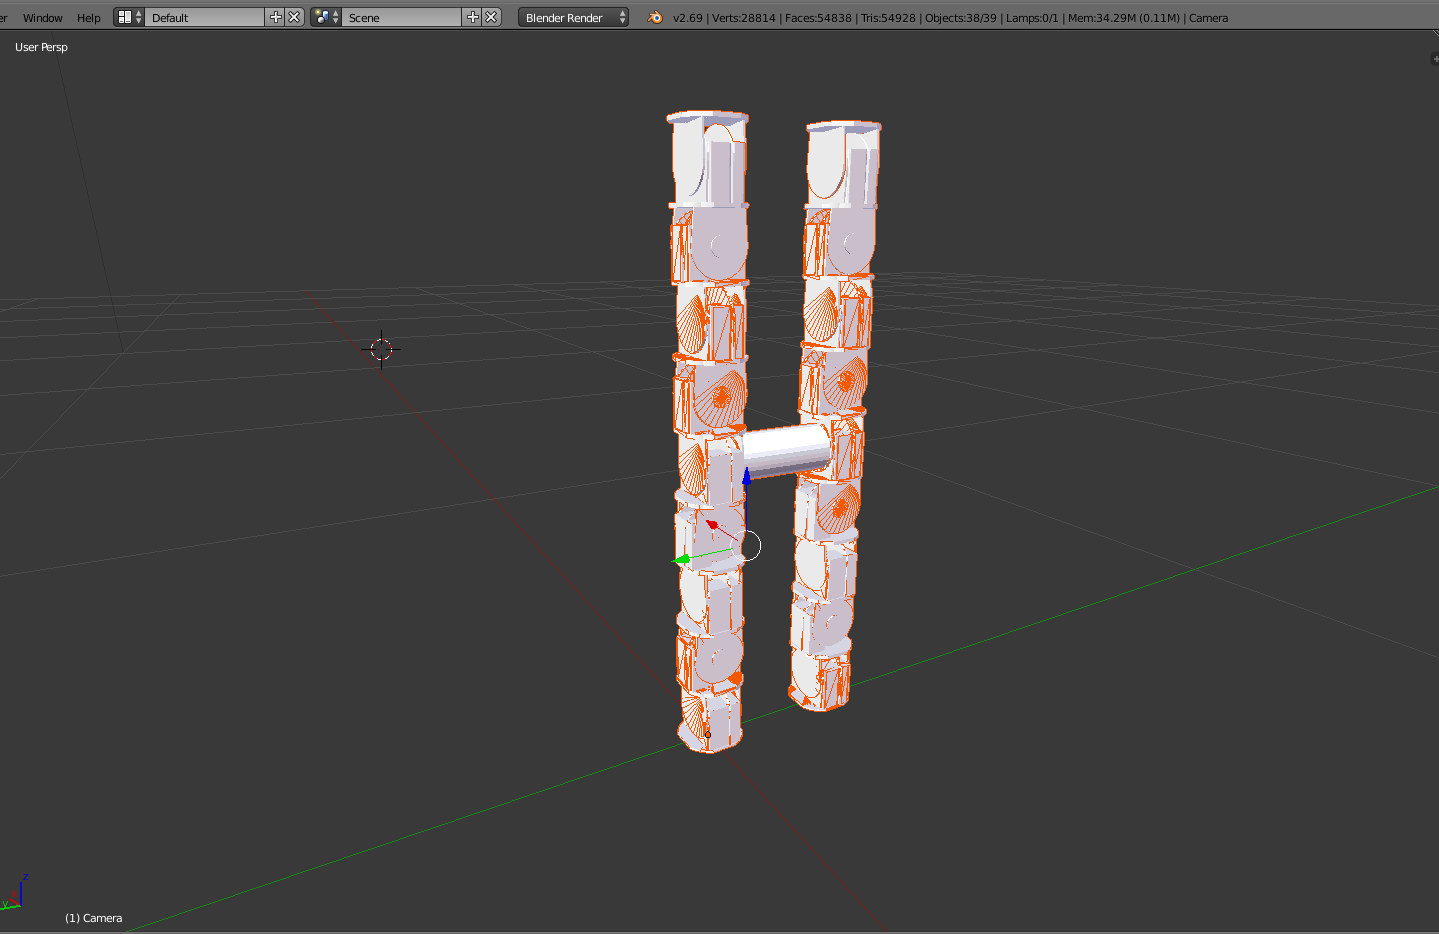
\includegraphics[scale=0.2]{screen_blender.png}
\caption{Progettazione su Blender del modello del robot}\label{fig:9}
\end{figure}

Il robot è poi stato importato nel programma di simulazione V-REP. Una volta importato, è stato necessario creare il modello dei moduli e quindi del robot completo definendo i punti di collisione, ovvero gli oggetti solidi che compongono il robot. Il modello di mesh infatti non possiede proprietà fisiche dell'oggetto, è compito del progettista (anche se si cerca di ricavarli in maniera automatica dalle mesh) generare i punti di collisione dalla mesh.
Una volta creati i punti di collisione, è stato verificato che il robot rimanesse in equilibrio statico; a causa della discretizzazione (e della creazione non molto precisa con Blender), il robot rimane in equilibrio statico ma tende a ``scivolare'' durante la simulazione. Purtroppo non è stato possibile aumentare il coefficiente di attrito dell'oggetto, quindi si ha una simulazione poco precisa.

In ambiente VREP poi sono stati aggiunti poi 1 sensore di visione da 64x64 px e 5 sensori di prossimità; il sensore di visione, posto sopra il robot, è stato impostato per vedere solo le fonti di calore (che rappresentano il target di movimento) e con una bassissima risoluzione, in modo da minimizzare il calcolo da parte dell'hardware riconfigurabile, mentre i sensori di prossimità hanno il fascio cilindrico e sono stati posti ad ogni lato del robot, leggermente sopraelevati rispetto alla base del robot in modo che i movimenti del robot non possano interferire con la rilevazione degli ostacoli.

\begin{figure}[htbp]
\centering
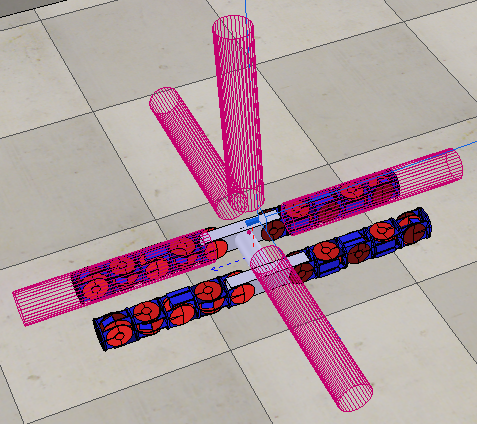
\includegraphics[scale=0.3]{tobor_sdraiato.png}
\qquad\qquad
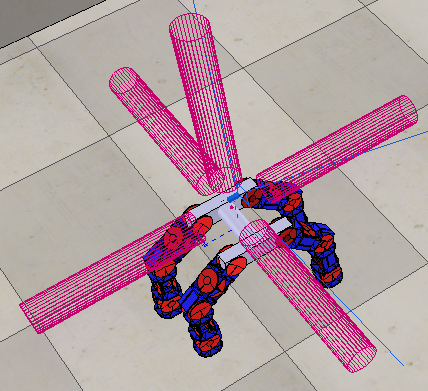
\includegraphics[scale=0.3]{tobor_quadrupede.png}
\caption{Robot nelle sue 2 configurazioni: a serpente doppio e a quadrupede}\label{fig:71}
\end{figure}

Dal punto di vista di controllo, il robot viene controllato in base alle posizioni dei giunti (controllo di posizione), quindi ogni istante della simulazione viene inviato un comando di posizione a tutti i giunti del robot per eseguire un movimento.
A causa della natura del sistema che lo comanda (hardware riconfigurabile), ogni posizione è discreta, quindi il moto non è stato descritto con un'equazione nel continuo ma da una serie di posizioni dei giunti.

Il robot è composto dalle seguenti parti:
\begin{itemize}
  \item diversi componenti locomotori connessi in maniera opposta l'uno dall'altro, che uniti tra loro permettono di eseguire molteplici movimenti;
  \item un corpo centrale a forma di ``H'', in cui risiede tutta la circuiteria e permette di avere una base solida per alcuni tipi di movimenti.
\end{itemize}

Ogni componente pesa $40g$ e deve avere l'attrito necessario per permettere il movimento; sfortunatamente il tool di simulazione non permette di impostarlo e quindi alcuni movimenti non rappresentano correttamente la realtà.

Per le diverse configurazioni, sono stati presi diversi modelli naturali per rappresentare il moto: la configurazione a serpente doppio ha preso spunto dal moto del serpente (moto ondulatorio verticale), mentre la configurazione a quadrupede ha preso spunto dalla marcia del cavallo (passo).

\subsection{Configurazione a serpente doppio}

In questa configurazione, il robot si trova sdraiato, completamente a contatto con il terreno. Per muoversi, deve eseguire un moto ondulatorio verticale, come alcuni tipi di serpenti. Questo tipo di moto può essere descritto con queste equazioni:

$$ y(t_{x}) = (j_{v1} \cdot (1-s)+j_{v2} \cdot s) \cdot \sin(t \cdot (v_{v1} \cdot (1-s)+v_{v2} \cdot s)+i \cdot (j_{v1} \cdot (1-s)+j_{v2} \cdot s)) $$
$$ y(t_{x+1}) = (j_{v1} \cdot (1-s)+j_{v2} \cdot s) \cdot \cos(t \cdot (v_{v1} \cdot (1-s)+v_{v2} \cdot s)+i \cdot (j_{v1} \cdot (1-s)+j_{v2} \cdot s)) $$

~

la variabile $ y $ indica l'output della funzione, $ t_{x} $ indica un istante di tempo generico mentre $ t_{x+1} $ indica l'istante di tempo successivo al precedente. Le variabili $ j_{v1}, j_{v2} $ indicano le posizioni dei giunti verticali, indipendentemente da quanti giunti esistono (come nel caso del tempo, si indicano semplicemente giunti successivi tra loro).  Le variabili $ v_{v1}, v_{v2} $ indicano invece le velocità dei giunti successivi tra loro.
Si deve pensare che queste 2 equazioni si devono eseguire ciclicamente in modo da avere un movimento continuo ed ondulatorio, per permettere di strisciare.

A causa della natura del robot, poichè la parte centrale è statica, si deve eseguire il movimento con più potenza del necessario, in modo da essere in un'istantanea fase di volo che può dare la spinta necessaria per avanzare (e quindi spostare la parte statica del robot).

Per la rappresentazione spaziale, è stato adottato il modello di \textit{Chirikjian - Burdick}, in cui si prende come sistema di riferimento fisso la ``cod'' del serpente, cioè l’ultimo giunto, e tutti i calcoli relativi ai successivi giunti del corpo serpentoide del robot verranno eseguiti in base a tale scelta. In particolare, il sistema viene visto come un insieme di 4 serpenti collegati ad un corpo rigido:
in questo modo i movimenti vengono semplicemente ripetuti in maniera speculare o come prolungamento di altri serpenti, semplicemente riferendosi ai giunti sequenziali del robot.

Poichè ogni posizione di ogni giunto è nota durante l'esecuzione, è stata utilizzata la cinematica diretta per determinare la posizione e il movimento di ogni componente. Inoltre, poiché il numero dei giunti era molto elevato, è stata utilizzata la convenzione di \textit{Denavit-Hartenberg}, rappresentando una trasformazione geometrica nello spazio euclideo tridimensionale con 4 parametri.
Calcolando questi valori, è stato possibile quindi calcolare la posizione dei giunti in maniera ottimale per il corretto movimento del robot.

Quindi, implementando ogni posizione dei giunti, si è riusciti a far muovere il robot con il moto ondulatorio verticale.

~

In questa configurazione è anche possibile muoversi lateralmente, rovesciando il robot lateralmente 2 volte consecutive. Per fare ciò, è necessario piegare contemporaneamente 2 giunti dello stesso lato, in modo che il robot si possa rovesciare nel lato opposto, per poi rieseguire lo stesso movimento con gli altri 2 giunti.

\subsection{Configurazione a quadrupede}

In questa configurazione, il robot si trova in posizione eretta sui suoi 4 arti che nella configurazione precedentemente descritta erano i 4 serpenti. Per questa configurazione non si è trovato un modello analitico per descrivere il moto del robot, quindi ci si è serviti dello studio cinematico di un cavallo, in particolare della cinematica del ``passo''.
Il passo è la camminata leggera del cavallo, che consiste nel muovere alternativamente e a coppie disallineati gli arti opposti, senza avere una fase di volo; in questo modo, si ha sempre la condizione di equilibrio una volta completato l'insieme di movimenti. La caratterstica di questo movimento però è lo sbilanciamento verso la direzione in cui ci si muove: gli arti vengono alzati in modo che avvenga uno sbilanciamento in avanti in modo che, raddrizzandoli successivamente, si è riusciti ad avanzare.

\begin{figure}[htbp]
\centering
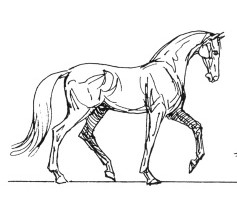
\includegraphics[scale=0.5]{cavallo_passo.jpg}
\qquad\qquad
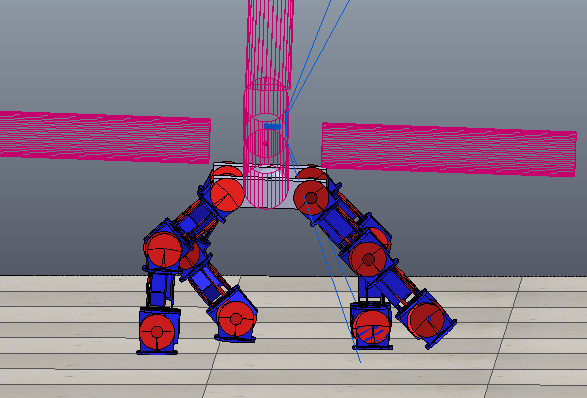
\includegraphics[scale=0.25]{passo1.png}
\caption{Confronto tra il ``passo'' del cavallo e il ``passo'' del robot}\label{fig:7}
\end{figure}

Per implementare il moto del robot quindi, è stato fatto uno studio cinematico del passo del cavallo, per poi riportare le posizioni dei ``giunti'' del cavallo nelle posizioni dei giunti del robot; in questo modo si è discretizzato il movimento del robot per poi permettergli di muoversi secondo un modello naturale funzionante, oltre a fare uno studio dell'anatomia del cavallo per capire come renderla compatibile con la configurazione a quadrupede del robot.
Utilizzando un controllo di posizione infine, si è riusciti facilmente ad implementare il corretto movimento: servendosi di uno studio di settore già stato eseguito \cite{robot_horse}, è stata semplicemente trascritta la posizione attesa dei giunti e rappresentata in simulazione.

\section{Intelligenza Artificiale}

Per completare il progetto, era necessario utilizzare un programma intelligente che potesse gestire il path planning; questo perché sarebbe troppo poco performante far eseguire il tutto all'hardware riconfigurabile, quindi si è implementato un programma esterno per gestire l'aspetto di pianificazione del percorso e il collision avoidance.

Il programma, scritto in C++, è in grado di interpretare i dati ricevuti dall'hardware riconfigurabile e prendere decisioni sul percorso da eseguire: i dati sono organizzati secondo un protocollo specifico, ovvero un ordine di segnali che corrispondono all'individuazione da parte di un sensore di un oggetto vicino. Il programma, sceglie il percorso durante l'avanzamento del robot nello spazio, memorizzando ad ogni passo la scelta eseguita; questo è molto importante per comprendere se durante il tragitto sono state fatte delle scelte sbagliate.
Il concetto di ``scelta sbagliata'' in questo contesto è semplice: se si ha una una situazione di impossibilità di movimento (il robot non può più eseguire l'azione che stava eseguendo, ci sono troppi ostacoli, ecc), allora il programma ha scelto un tragitto sbagliato. Dal momento che il programma si rende conto che ha commesso un errore di scelta, deve essere in grado di capire quando è stato fatto lo sbaglio, ovvero deve tornare indietro eseguendo i tutti i movimenti al contrario fino all'ultimo movimento errato,
ovvero quando ha iniziato a fare il movimento che l'ha portato nella situazione errata. Alla fine dell'esecuzione, il programma ha mantenuto la lista di comandi che hanno portato il robot a raggiungere l'obbiettivo, quindi la stessa lista si potrebbe utilizzare potenzialmente per eseguire il percorso senza commettere errori.

Il programma implementa quindi la tecnica di \textit{A Star} con la variante \textit{Fog War and no path information}: si utilizza un'euristica per raggiungere la fonte di calore, ovvero mantenere centrata la fonte di calore nel visualizzatore, senza però sapere com'è fatto il percorso, avvolto quindi da una ``nebbia di guerra'' che impedisce di sapere cosa si trova dinanzi. Il concetto di nebbia di guerra è stato importato dai videogiochi e quindi dall'intelligenza artificiale dei personaggi,
in quanto in alcuni tipi di giochi strategici è stata implementata una mappa le cui informazioni interne non sono note, devono essere scoperte dal videogiocatore o dal nemico virtuale (che quindi deve viaggiare nella mappa pur non sapendo che ostacoli può trovare).
La tecnica dell' A star si è dimostrata molto efficace, in quanto il percorso risulta discretizzato in base ai movimenti possibili del robot e la visione della mappa viene modificata dalle 2 configurazioni. Si può pensare quindi di avere una mappa a 2 livelli, i quali possono essere sostituiti a piacere in base alla situazione.

\begin{figure}[htbp]
\centering
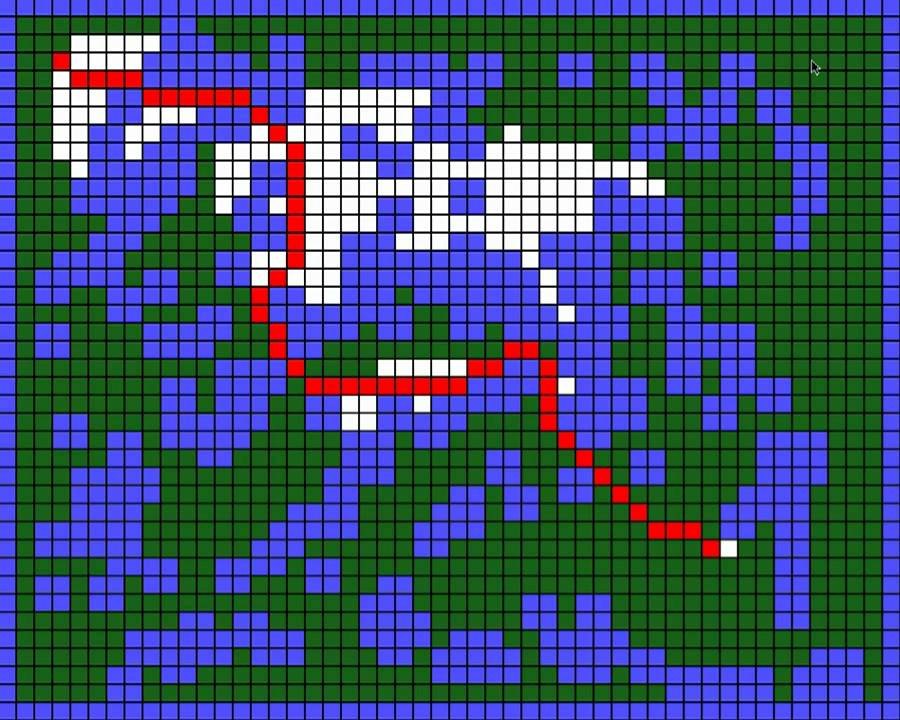
\includegraphics[scale=0.3]{a_star.jpg}
\caption{Mappa in cui utilizzare A Star (percorso in rosso, ostacoli in verde, ostacoli in bianco oltrepassabili strisciando)}\label{fig:8}
\end{figure}

\subsection{Algoritmo}

L'algoritmo intelligente definisce una serie di regole che il robot deve adottare in modo da trovare il percorso corretto per raggiungere l'obbiettivo. Questo quindi consisterà in una serie di letture dei dati derivanti dai sensori, che verranno interpretati e quindi si deciderà quale azione eseguire. Da notare che l'ordine dei controlli è molto importante: si definisce una priorità di controlli in modo che, a parità di configurazione, la priorità delle scelte possa cambiare l'esecuzione del programma.
Il programma sarà sempre sincronizzato con il sistema sottostante, non ha visione del mondo che lo circonda ma semplicemente interpreta tramite regole prestabilite i segnali che arrivano dai sensori. Infine, deve essere un algoritmo semplice e che non richieda troppo utilizzo di memoria e risorse, in quanto deve essere più veloce possibile e calato in un contesto di un microcontrollore che si trova a bordo del robot, quindi indubbiamente con non ottime capacità di calcolo.

\begin{algorithm}[H]
 \KwData{Robot input}
 \KwResult{Movement decisions}
 initialization\;
 \While{not arrived}{
    read current data\;
    \uIf{I can go ahead}{
      go ahead\;
     }
    \uElseIf{I can go ahead but I'm lying}{
      go ahead dragging\;
    }
    \uElseIf{I'm under the obstacle}{
      go ahead dragging\;
      memorize that I'm under the obstacle\;
   }
   \uElseIf{I'm not under the obstacle}{
     go ahead dragging\;
     memorize that I'm not under the obstacle\;
   }
   \uElseIf{I can get up}{
     get up\;
   }
   \uElseIf{I can't go ahead for an obstacle}{
     crouch\;
   }
   \uElseIf{I can't go ahead lying (try to go right)}{
     go right\;
     memorize that I'm going right\;
   }
   \uElseIf{I can't go ahead lying (try to go left)}{
    go left\;
    memorize that I'm going left\;
   }
   \uElseIf{I can't try another movement to right}{
    rollback actions\;
   }
   \uElseIf{I can't try another movement to left}{
    rollback actions\;
   }
   \uElse{
    I don't know, abort\;
   }
 }
\caption{Algoritmo di path planning del robot}
\end{algorithm}


\begin{thebibliography}{1}
\bibitem{MS1} Garrison W. Greenwood,Senior Member, IEEE and Andy M. Tyrrell,Senior Member, IEEE, ``\textit{Metamorphic Systems: A New Model for Adaptive System Design''}, 2010
\bibitem{EIE} Sekanina, L. ; Brno Univ. of Technol., Brno ; Martinek, T. ; Gajda, Z., \textit{Extrinsic and Intrinsic Evolution of Multifunctional Combinational Modules}, 2006
\bibitem{PR1} Altera, \textit{FPGA Run-Time Reconfiguration: Two Approaches}, 2008
\bibitem{PR2} Dirk Koch, \textit{Partial Reconfiguration on FPGAs}, 2013
\bibitem{Rechannel} Raabe A., Tech. Comput. Sci., Univ. of Bonn, Felke A., \textit{A SYSTEMC language extension for high-level reconfiguration modelling}, 2008
\bibitem{Rechannel2} Erlangung des Doktorgrades, Mathematisch-Naturwissenschaftlichen Fakultat, Rheinischen Friedrich-Wilhelms-Universitat Bonn, \textit{Describing and Simulating Dynamic Reconfiguration in SystemC Exemplified by a Dedicated 3D Collision Detection Hardware}, 2008
\bibitem{robot_syntax} Masahiro Fujita Hiroaki Kit an0 Toshitada Doi, \textit{Syntactic-Semantic Analysis of Reconfigurable Robot}, 1999
\bibitem{robot_horse} S.Makita, N.Murakami, M.Sakaguchi, J.Furusho, \textit{Development of Horse-type Quadruped Robot}, 1999
\end{thebibliography}

\end{document}
